\chapter{C\'alculo diferencial (algebraico)}
\section{Derivaciones}
Sea $k$ un anillo (frecuentemente, un cuerpo) y $A$ una $k$-\'algebra ($k \to A$ morfismo de anillos, de forma que para $\lambda \in k$ se denota $\lambda \in A$). Sea $M$ un $A$-m\'odulo (por tanto $k$-m\'odulo).
\begin{defi}
    Una derivaci\'on de $A$ en $M$ sobre $k$ (\'o trivial sobre $k$) es una aplicaci\'on
    $\bt D: A \rar & M  \et$ cumpliendo \vspace{-3mm}
    \begin{enumerate}
        \item $k$-lineal ($D(\lambda a) = \lambda Da$)
        \item Regla de Leibnitz: $D(ab) = aDb + bDa \, \forall \, a,b \in A$.
    \end{enumerate}
    Se denota $Der_k(A,M)$ al conjuto de derivaciones de $A$ en $M$ sobre $k$. 
\end{defi}
\begin{prop}
    $Der_k(A,M)$ tiene estructura de $A$-m\'odulo.
\end{prop}
\begin{dem}
    Se tiene que para dos derivaciones $D, \, D'$, 
    \begin{enumerate}
        \item $D+ D': A\longrightarrow M$ es tal que $(D+D')(a) \coloneq Da+D'a$, que cumple ambas condiciones:
        \begin{enumerate}
            \item $(D+D')(\lambda a)= D(\lambda a) + D'(\lambda b) = \lambda Da+\lambda D'a=\lambda (Da+D'a)=\lambda (D+D')(a)$
            \item $(D+D')(ab) = Dab + D'ab = aDb + bDa + aD'b + bD'a = $ \\ 
            $ \hspace{15mm}   = aDb+aD'b+bDa+bD'a = a(D+D')(b) + b (D+D')(a)$
        \end{enumerate}
        \item $aD : A \longrightarrow M$ es tal que $(aD) (a') \coloneq a \cdot Da'$, que cumple ambas condiciones.
    \end{enumerate}
    y con esta suma y este producto cumple los axiomas de $A$-m\'odulo. 
\end{dem}
\begin{prop}
    $D$ se anula sobre $k$. 
    $D \lambda = 0 \, \forall \, \lambda \in k$. 
\end{prop}
\begin{dem} Usando que $D$ es $k$-lineal;
$$D\lambda = D(\lambda \cdot 1) = \lambda D(1) = 0$$
pues 
$$D1 = D(1\cdot 1) = D1 + D1 \iff D1=0 $$
\end{dem}
\begin{prop}
    Sea $f:M \longrightarrow N$ un morfismo de $A$-m\'odulos, 
    $$\bt A \rar{D} \arrow[swap]{dr}{f\circ D} & M\arrow{d}{f} \\ & N \et$$
    $f\circ D: A \longrightarrow N$ es una derivaci\'on. 
\end{prop}
Tenemos pues una aplicaci\'on
$$\bt Der_k(A,M) \rar{f_*}&  Der_k(A,N) \\[-5mm] D \rarmaps & f\circ D \et$$
que es morfismo de $A$-m\'odulos. Para todo morfismo $N \overset{g}{\longrightarrow} P$, $g_* \circ f_* = (g\circ f)_*$, y con $Id_* = Id$. 

As\'i pues, tenemos el funtor 
$$\bt \{A-mod\} \rar{Der_k(A,-)} & \{A-mod\} \\[-5mm] M \arrow{dd}{f} & Der_k(A,M) \arrow[swap]{dd}{f_*} \\[-3mm] \, \, \, \, \, \, \,  \arrow[squiggly]{r} & \, \, \, \, \, \, \, \, \,  \\[-3mm] N & Der_k(A,N)  \et$$
y es representable por
$$Der_k(A,-) = Hom_A(\Omega_{\nicefrac{A}{k}}, -)$$
\begin{propi}
    Sea $h: A \longrightarrow A'$ un morfismo de $k$-\'algebras, consideremos $M$ un $A'$-m\'odulo (por tanto $A$-m\'odulo). Si tenemos una derivaci\'on de $A'$ en $M$, al componerla con este morfismo
    $$\bt A\arrow[bend right=15mm]{rr}{D\circ h} \rar{h} & A' \rar{D} & M \et$$
    es una derivaci\'on de $A$.
\end{propi}
\begin{cor}
        Tenemos as\'i una aplicaci\'on $Der_k(A',M) \longrightarrow Der_k(A,M)$
\end{cor}
\begin{propi}
    Sea ahora $k \longrightarrow k'$ un morfismo de anillos, $A_{k'} = A \underset{k}{\otimes} k'$ es una $k'$-\'algebra, con el diagrama
    $$\bt k\arrow{d} \rar &  A \arrow{d} \\k' \rar & A_{k'} \et$$
    Si tenemos un $A$-m\'odulo $M$, 
    $$M  \underset{A}{\otimes} A_k = M  \underset{A}{\otimes} A  \underset{k}{\otimes} k' = M  \underset{k}{\otimes} k' \coloneq M_{k'}$$
    es tambi\'en $k'$-m\'odulo.

    Todo esto nos dice que si tenemos $D: A \longrightarrow M$, se induce una derivaci\'on 
    $A_{k'} \longrightarrow M_{k'}$, y se denota por $D\otimes 1$, definida por
    $$\bt D \otimes 1: &[-12mm]  A \underset{k}{\otimes} k' \rar & M  \underset{k}{\otimes} k'\\[-5mm]
        &[-5mm] a \otimes \eta \rarmaps & Da \otimes \eta 
    \et$$
    por lo que tenemos 
    $$\bt Der_k(A,M) \rar & Der_{k'}(A_{k'},M_{k'}) \\[-5mm] D \rarmaps & D\otimes 1 \et$$
\end{propi}
\section{M\'odulo de diferenciales de Kähler de $A$ sobre $k$: $\Omega_{\nicefrac{A}{k}}$}
Dado $k \longrightarrow A \overset{p}{\longrightarrow} k$, llamaremos ``puntos de $A$ (con valores en $k$)'' a $p: A \longrightarrow k$ un morfismo de $k$-\'algebras, y diremos $\Omega_{\nicefrac{A}{k},p} = \modulo{I_p}{I_p^2}$ siendo $I_p = \ker(A \overset{p}{\longrightarrow} k)$. 

Si $k$ es cuerpo, $p$ es epiyectivo e $I_p$ ser\'ia un ideal maximal. 

Si $A$ es $k$-\'algebra, $$ \bt k\arrow[bend right=10mm]{rr} \rar[hook] &  A \rar & \modulo{A}{\m} \et$$
de forma que puede ser que $\modulo{A}{\m} = k$, y en ese caso diremos que el punto sobre el que trabajamos $p$ es un punto racional.

Sea ahora $A \overset{p}{\longrightarrow} \bar k$ un morfismo de $k$-\'algebras, siendo $k \subset \bar k$. Interpretamos esto como un punto de $A$ con valores en $\bar k$. Tenemos $k \longrightarrow \bar k$, y por tanto
$$\bt A  \underset{k}{\otimes} \bar k \rar & \bar k \\[-5mm] a\otimes \eta \rarmaps & p(a) \cdot \eta \et$$
con un cierto n\'ucleo $I_{p\otimes 1}$, que es algo que ya sabemos, por el cambio de base
$$\bt Hom_{k-alg}(A, \bar k) \rar[equal] & Hom_{\bar k-alg}(A \underset{k}{\otimes} \bar k, \bar k) \\[-5mm] p \rarmaps & p\otimes 1 \et$$
de forma que hemos convertido en racional el punto $p$. As\'i, 
$$\Omega_{\nicefrac{A}{k}, p} = \modulo{I_{p\,\otimes 1}}{I^2_{p\, \otimes 1}}$$
 

\justifying
\section{Diferenciales}
Sea $A$ una $k$-\'algebra ($k \to A$).
\begin{defi}
    El morfismo diagonal es una aplicaci\'on
    $$\bt A \underset{k}{\otimes} A \rar & A \\[-8mm] a\otimes a' \rarmaps & a\cdot a'  \et$$
    que verifica ser inyectivo y morfismo de $k$-\'algebras (de anillos en particular).
\end{defi}
\begin{obs}    
    Llamando $\Delta = $ n\'ucleo del morfismo diagonal:
    $$\bt 0 \rar & \Delta \rar & A \underset{k}{\otimes} A \rar & A \rar & 0 \et$$
    es sucesi\'on exacta, y tenemos dos morfismos
    $$\bt A \rar[shift left=1mm] \rar[shift right=1mm] & A \underset{k}{\otimes} A \\[-8mm] a \rarmaps & a\otimes 1 \\[-5mm] a \rarmaps & 1\otimes a  \et$$
    que es lo que llamamos m\'odulos por la izquierda o por la derecha. En general, consideraremos la estructura de m\'odulo por la derecha (pues esta segunda $A$ act\'ua como un cambio de base).

    Adem\'as, la sucesi\'on exacta es de $A$-m\'odulos y rompe, pues $A \underset{k}{\otimes} A \to A$ tiene secci\'on, como acabamos de ver. 
\end{obs}
\begin{defi}
    $\Omega_{\nicefrac{A}{k}} \coloneq \modulo{\Delta}{\Delta^2} $. 
\end{defi}
\begin{prop}
    $\modulo{\Delta}{\Delta^2} = \Delta \underset{A \underset{k}{\otimes} A}{\otimes} \modulo{(A \underset{k}{\otimes} A)}{\Delta}$
\end{prop}
\begin{dem}
    Usando que para todo ideal $I \subset A, \, \modulo{I}{I^2} = I \underset{A}{\otimes} \modulo{A}{I}$, y adem\'as, $\modulo{(A \underset{k}{\otimes} A)}{\Delta} = A$
\end{dem}
\section{La diferencial}
\begin{defi}
    La diferencial es una aplicaci\'on $d: A \longrightarrow \Omega_{\nicefrac{A}{k}}$, una derivaci\'on de $A$ en $\Omega_{\nicefrac{A}{k}}$ sobre $k$. 
    $$\bt A \arrow[bend left=10mm]{rrr}{d} \rar{\delta} & \Delta\arrow{rr} &[-13mm] &[-8mm]  \modulo{\Delta}{\Delta^2} = \Omega_{\nicefrac{A}{k}} \\[-10mm] a \rarmaps &[-13mm] \delta a \coloneq &[-8mm] a\otimes 1 - 1 \otimes a \\ & &[-18mm] &[-8mm]  da = \overline{\delta a} = \overline{a\otimes 1 - 1 \otimes a}\et$$
\end{defi}
\begin{prop}
    $\Delta$ est\'a generado por los $\delta a$ (como $A$-m\'odulo). 
\end{prop}
\begin{dem}
    Sea $\Delta = \ker(A \underset{k}{\otimes} A \to A)$. Un elemento de $A \underset{k}{\otimes} A$ es $\sum a_i \otimes b_i$ finita, y por el morfismo diagonal,$\sum a_i \otimes b_i \longrightarrow \sum a_i b_i$, y $\sum a_i \cdot  b_i = 0$ si $\sum a_i \otimes b_i \in \Delta$. De forma que
    $$\sum a_i \otimes b_i = \sum a_i \otimes b_i- 1\otimes \underbrace{\sum a_i \cdot b_i}_{=0} = \sum (a_i \otimes b_i - 1\otimes a_i b_i) = \sum b_i (\delta a_i)$$
\end{dem}
\begin{cor}
    $\Omega_{\nicefrac{A}{k}}$ est\'a generado (como $A$-m\'odulo) por los $da$. Es decir, todo elemento de $\Omega_{\nicefrac{A}{k}}$ es de la forma
    $$\sum b_i \cdot da_i$$
    siendo una suma finita. 
\end{cor}
\begin{prop}
    La diferencial $d: A \longrightarrow \Omega_{\nicefrac{A}{k}}$ es una derivaci\'on de $A$ en $\Omega_{\nicefrac{A}{k}}$ sobre $k$.
\end{prop}
\begin{dem}
\begin{enumerate}
    \item Es $k$-lineal por ser composici\'on de aplicaciones $k$-lineales. 
    \item Leibnitz: $d(ab) = bda + adb$
    $$d(ab) = \overline{ab \otimes 1 - 1 \otimes ab} = \cdots \mod \Delta^2$$
    \begin{align*}
        b \, da+ a\,  db = & b (\overline{a\otimes 1 - 1 \otimes a}) + a (\overline{b\otimes 1 - 1 \otimes b}) = \\
        = &  \overline{b(a\otimes 1 - 1 \otimes a) + a (b\otimes 1 - 1 \otimes b)} = \overline{a\otimes b -1 \otimes ab + b \otimes a - 1\otimes ab}
    \end{align*}
    y veamos que son representantes de la misma clase, es decir, que 
    $$ab \otimes 1 - \cancel{1 \otimes ab} - (a\otimes b -1 \otimes ab + b \otimes a - \cancel{1\otimes ab}) \in \Delta^2$$
    $$= (a\otimes 1 - 1\otimes a) (b \otimes 1 - 1 \otimes b) = (\delta a) \cdot (\delta b)$$
    y como $\delta a \in \Delta$ y $\delta b \in \Delta$, entonces $(\delta a)(\delta b) \in \Delta^2$. 
\end{enumerate}
\end{dem}
As\'i pues, hemos construido $d$ y $\Omega_{\nicefrac{A}{k}}$, de forma que para todo $A$-m\'odulo $M$, 
$$\bt Hom_{A}(\Omega_{\nicefrac{A}{k}}, M ) \rar &  Der_k(A, M) \\[-5mm] f\rarmaps & f\circ d \et$$
es un morfismo de $A$-m\'odulos.
\begin{teo}
    $\bt Hom_{A}(\Omega_{\nicefrac{A}{k}}, M ) \rar &  Der_k(A, M) \et$ es isomorfismo $\forall M \in A\mathbf{-mod}$. 
\end{teo}
\begin{dem}
    Construyamos la aplicaci\'on inversa. Dada $D : A \longrightarrow M$ (una derivaci\'on sobre $k$), $i_D : \Omega_{\nicefrac{A}{k}} \longrightarrow M$ morfismo de $A$-m\'odulos. 

    Tenemos la aplicaci\'on
    $$\bt D\otimes 1: A\underset{k}{\otimes} A \rar & M \\[-8mm] a\otimes b \rarmaps & b \cdot Da \et $$
    que es morfismo de $A$-m\'odulos. Tenemos $\Delta \subseteq  A\underset{k}{\otimes} A$, de forma que tenemos $D\otimes 1|_{\Delta} : \Delta \longrightarrow M$ y si se anula sobre $\Delta^2$ factoriza por $\modulo{\Delta}{\Delta^2}$, es decir, se tendr\'ia el siguiente diagrama
    $$\bt  A\underset{k}{\otimes} A \rar{D\otimes 1} & M \\ \Delta \arrow[ u , phantom,  "\rotatebox{90}{$\subseteq$}"] \arrow{ur}{D\otimes 1} \arrow{r} & \modulo{\Delta}{\Delta^2} \arrow{u}{i_D} \et$$
    
    
    En efecto, $D\otimes 1$ se anula sobre $\Delta^2$., pues $\Delta^2$ est\'a generado por elementos de la forma $\delta a \cdot \delta b$, luego veamos si $(D\otimes 1)(\delta a \delta b) =0$.
    \begin{align*}
        \delta a \cdot \delta b = a\otimes b -1 \otimes ab + b \otimes a -1\otimes ab
    \end{align*}
    luego aplicando $D\otimes 1$
    \begin{align*}
        (D\otimes 1)(a\otimes b -1 \otimes ab + b \otimes a -1\otimes ab) = & D(ab) - bDa - aDb + ab\cancelto{0}{D1} = 0
    \end{align*}
    por la regla de Leibnitz.

    Veamos que $D \longmapsto i_D \longmapsto i_D \circ d = D$, aplicando a un $a$,
    $$i_D(da) = (i_D\circ d)(a) = Da$$
    pues 
    $$i_D(da) = i_D(\overline{\delta a}) = (D\otimes 1)(\delta a) = (D\otimes 1)(a\otimes 1 - 1 \otimes a) = Da - aD1 = Da$$

    Adem\'as, $f \longmapsto f\circ d \longmapsto i_{f\circ D} = f$, basta ver que $i_{f\circ d}(da) = (f\circ d)(a) = f(da)$ (usar con cuidado las definiciones). 
\end{dem}

Tenemos la correspondencia
$$\bt Hom_A (\Omega_{\nicefrac{A}{k}}, M )\rar[equal] & Der_k(A,M) \\[-5mm] f \rarmaps&  f\circ d \\[-5mm] i_D & \arrow[mapsto]{l} D \et$$
y para $D \longmapsto i_D \longmapsto i_D \circ D$ se cumple que $i_D(da) = Da$. De modo contrario, $f \longmapsto f\circ d \longmapsto i_{f\circ d} \overset{?}{=}f$, $i_{f\circ d}(da) = (f\circ d)(a) = f(da)$ que es cierto usando lo anterior. 


Tenemos as\'i que es funtorial, es decir, para cada $h: A \longrightarrow B$ morfismo de $k$-\'algebras el siguiente diagrama
$$\bt da \rarmaps & d(ha) \\[-7mm] \Omega_{\nicefrac{A}{k}} \rar & \Omega_{\nicefrac{B}{k}}  \\ A \arrow{u}{d_A} \rar{h} & B \arrow{u}{d_B} \et$$
es conmutativo. Adem\'as $\bt\Omega_{\nicefrac{A}{k}} \rar & \Omega_{\nicefrac{B}{k}} \et$ es morfismo de $A$-m\'odulos (y derivaci\'on por ser $d_B \circ h$ una derivaci\'on). Como $\Omega_{\nicefrac{B}{k}}$ es $B$-m\'odulo, podemos cambiar de base y asegurar que $\bt\Omega_{\nicefrac{A}{k}} \underset{A}{\otimes} B \rar & \Omega_{\nicefrac{B}{k}} \et$ es morfismo de $B$-m\'odulos.

Tenemos que $$\bt k \rar \arrow{dr} & A\arrow{d} \\ & \modulo{A}{\m} \et$$ y si $\m$ es un ideal (maximal si es cuerpo)
\begin{teo}
    $\Omega_{\nicefrac{A}{k}} \underset{A}{\otimes} \modulo{A}{\m} = \modulo{\m}{\m^2}$
\end{teo}
\begin{dem}
    Se tiene la sucesi\'on exacta
    $$\bt 0\rar &  \Delta \rar & A \underset{k}{\otimes} A \rar &  A \rar & 0\et$$
    y escindida de $A$-m\'odulos. Luego tensorializamos por $\modulo{A}{\m}$, y se mantiene la exactitud al ser escindida, es decir
    $$\bt 0\rar & \Delta \underset{A}{\otimes} \modulo{A}{\m} \rar & (A \underset{k}{\otimes} A)\underset{A}{\otimes} \modulo{A}{\m} \rar & \modulo{A}{\m} \rar & 0\et$$
    donde $(A \underset{k}{\otimes} \cancel{A})\underset{\cancel{A}}{\otimes} \modulo{A}{\m} = A\underset{k}{\otimes} \modulo{A}{\m} = A$, de forma que la sucesi\'on es
    $$\bt 0\rar &  \m \rar & A \rar &  \modulo{A}{\m} \rar & 0\et$$
    y $\Delta \underset{A}{\otimes} \modulo{A}{\m} = \m$ aparece por ser el n\'ucleo de $A \longrightarrow \modulo{A}{\m}$. 

    Por tanto, $\modulo{\Delta}{\Delta^2} \underset{A}{\otimes} \modulo{A}{\m} = \modulo{\m}{\m^2}$ que sale al usar la sucesi\'on exacta
    $$\bt 0\rar &  \Delta^2 \rar & \Delta \rar &  \Omega_{\nicefrac{A}{k}} \rar & 0\et$$
    y al tensorializar por $\underset{A}{\otimes} \modulo{A}{\m}$, obtenemos el resultado, aunque perdemos la inyectividad.
\end{dem}
\begin{teo}[de cambio de base]
    Sea $k \longrightarrow A$ una $k$-\'algebra y $k'\longrightarrow A$ una $k'$-\'algebra, con $A_{k'} = A \underset{k}{\otimes} k'$. Se cumple que 
    $$\Omega_{\nicefrac{A}{k}} \underset{A}{\otimes} A_{k'} = \Omega_{\nicefrac{A}{k}} \underset{k}{\otimes} k' = \Omega_{\nicefrac{A_{k'}}{k}}$$
\end{teo}
\begin{dem}
    Se tiene la sucesi\'on exacta escindida de $A$-m\'odulos 
    $$\bt 0\rar &  \Delta \rar & A \underset{k}{\otimes} A \rar &  A \rar & 0\et$$
    luego de $k$-m\'odulos escindida y tensorializando, $\underset{k}{\otimes} k'$ sigue siendo exacta, luego
    $$\bt 0\rar &  \Delta \underset{k}{\otimes} k' \rar & A \underset{k}{\otimes} A\underset{k}{\otimes} k' \rar &  A\underset{k}{\otimes} k' \rar & 0\et$$
    es 
    $$\bt 0\rar & \Delta \underset{k}{\otimes} k' \rar & A_{k'} \underset{k'}{\otimes} A_{k'}  \rar &  A_{k'} \rar & 0\et$$
    y tenemos el morfismo diagonal en $k'$, y 
    $$\bt 0\rar &  \Delta' \rar & A_{k'} \underset{k'}{\otimes} A_{k'}  \rar &  A_{k'} \rar & 0\et$$
    de forma que $\Delta' = \Delta \underset{k}{\otimes} k'$ de forma que esta igualdad nos asegura que $$\modulo{\Delta}{\Delta^2} \underset{k}{\otimes} k' = \modulo{\Delta'}{(\Delta')^2}$$
    siguiendo el mismo argumento que en la demostraci\'on anterior. 
\end{dem}
\begin{custom}[1ª Sucesi\'on exacta de diferenciales] Sean las \'algebras $k \longrightarrow A \longrightarrow B$ ($A$ es $k$-\'algebra, $B$ es $A$-\'algebra y $k$-\'algebra), se tiene la sucesi\'on exacta
    $$\bt  \Omega_{\nicefrac{A}{k}} \underset{A}{\otimes} B \rar & \Omega_{\nicefrac{B}{k}} \rar &  \Omega_{\nicefrac{B}{A}} \rar & 0\et$$
\end{custom}
\begin{dem}
    Tenemos $\bt B \rar{d_{\nicefrac{B}{A}}} & \Omega_{\nicefrac{B}{A}} \et$ que es $A$-lineal, en particular $k$-lineal. De forma que el morfismo $ \Omega_{\nicefrac{B}{k}} \longrightarrow  \Omega_{\nicefrac{B}{A}}$ es la \'unica que hace conmutativo el siguiente diagrama
    $$\bt B \rar{d_{\nicefrac{B}{A}}}  \arrow[swap]{d}{d_{\nicefrac{B}{k}}} & \Omega_{\nicefrac{B}{A}} \\ \Omega_{\nicefrac{B}{k}} \arrow{ru} & d_{\nicefrac{B}{A}}b \\[-5mm] d_{\nicefrac{B}{k}} b \arrow[mapsto]{ru}  \et$$
    y es exacta pues al tomar $Hom_B$ lo es:
    $$\bt 0 \rar & Hom_B(\Omega_{\nicefrac{B}{A}}, M) \rar &  Hom_B(\Omega_{\nicefrac{B}{k}}, M) \rar &  Hom_B(\Omega_{\nicefrac{A}{k}} \underset{A}{\otimes} B, M) \\[-5mm] 
    & & & Hom_A(\Omega_{\nicefrac{A}{k}}, M )\arrow[equal]{u} \\[-5mm] 
    0 \rar & Der_A(B, M) \arrow[equal]{uu}  \rar[hook]  & Der_k(B, M) \arrow{r} \arrow[equal]{uu} & Der_k(A, M) \arrow[equal]{u} \\[-5mm] 
    & D \rarmaps & D \arrow[mapsto]{r} & D \circ h  \et$$
    y como $D$ se anula sobre $A$, esto es que $D(ab) = b \, \cancelto{0}{Da}+ a \, Db = a \,Db$ es $A$-lineal, luego es un elemento de $Der_A(B,M)$. 
\end{dem}
\begin{custom}[2ª Sucesi\'on exacta de diferenciales] 
    Tenemos las \'algebras $k \longrightarrow A \longrightarrow \modulo{A}{I}$, de forma que $\Omega_{\nicefrac{A}{k}} \underset{A}{\otimes} \modulo{A}{I}$ y $\Omega_{\nicefrac{\nicefrac{A}{I}}{k}}$ forma la sucesi\'on exacta
    $$\bt  \modulo{I}{I^2} \rar & \Omega_{\nicefrac{A}{k}} \underset{A}{\otimes} \modulo{A}{I}  \rar & \Omega_{\nicefrac{(\nicefrac{A}{I})}{k}} \rar & 0 \\[-7mm] [i] \rarmaps & \overline{di} = di \otimes 1 \et$$
    pues podemos pensar $ \Omega_{\nicefrac{A}{k}} \underset{A}{\otimes} \modulo{A}{I} =\modulo{\Omega_{\nicefrac{A}{k}}}{I\cdot \Omega_{\nicefrac{A}{k}}}$, y esta asignaci\'on no depende del representante escogido. Adem\'as la primera aplicaci\'on es morfismo de $\modulo{A}{I}$-m\'odulos, con 
    $$[a]\cdot [i] = [a\cdot i] \longmapsto \overline{d(ai)} = \overline{a \, di + d \cancel{da}} = \overline{a} \cdot \overline{di}$$ 

    Tomando $Hom$ en la sucesi\'on sobre $M$ cualquier $\modulo{A}{I}$-m\'odulo:
    $$\bt  
    Hom_{\nicefrac{A}{I}}(\Omega_{\nicefrac{(\nicefrac{A}{I})}{k}}, M) \rar &  Hom_{\nicefrac{A}{I}}\left(\Omega_{\nicefrac{A}{k}} \underset{A}{\otimes} \modulo{A}{I}, M\right)  \rar &  Hom_{\nicefrac{A}{I}}\left(\modulo{I}{I^2},M\right) \rar & 0 \\[-5mm] 
    & Hom_{A}(\Omega_{\nicefrac{A}{k}}, M ) \arrow[equal]{u}  \\[-5mm] 
    Der_k\left(\modulo{A}{I}, M\right) \arrow[equal]{uu} \rar & Der_k(A,M) \arrow[equal]{u} \rar  & Hom_A(I,M) \arrow[equal]{uu} \\[-5mm] D \rarmaps & D\circ \pi \\[-5mm] & D:A\to M \rarmaps & D|_{I} \et$$
    y teniendo en cuenta que $\modulo{I}{I^2} = I \underset{A}{\otimes} \modulo{A}{I}$, y con el diagrama $$\bt  A \rar{D} \arrow{d} & M \\[3mm] \modulo{A}{I} \arrow[swap]{ru}{\bar D} \et$$ obtenemos las diferenciales de $\modulo{A}{I}$.
\end{custom}
\begin{cor}
    Esta sucesi\'on exacta nos dice que sabiendo $\Omega_{\nicefrac{A}{k}}$ para saber las diferenciales de $\modulo{A}{I}$, tenemos que hacer m\'odulo por el ideal $I$ y las diferenciales del ideal, es decir, $\Omega_{\nicefrac{A}{k}} \underset{A}{\otimes} \modulo{A}{I} = \modulo{\Omega_{\nicefrac{A}{k}}}{I \cdot \Omega_{\nicefrac{A}{k}}}$. 
\end{cor}
\begin{ejem}
    Sea $k \to k[x]$ la $k$-\'algebra, se tiene que $\pdd{}{x} : k[x] \to k[x]$ es una derivaci\'on dada por $\pdd{}{x}(x^n) = n x^{n-1}$. Esto es, para todo $\pdd{}{x} \left(\sum \lambda_i x^i \right) = \sum \lambda_i \, i\, x^{i-1}$, para cualquier $P \in k[x]$, $\pdd{P}{x} = P'$. 
\end{ejem}
\begin{prop}
    $\Omega_{\nicefrac{k[x]}{k}} = k[x] \cdot dx$, es decir, veamos que $\Omega_{\nicefrac{k[x]}{k}}$ es libre de base $dx$.
\end{prop}
\begin{dem}    
    Se tiene que $k[x] \overset{d}{\longrightarrow} \Omega_{\nicefrac{k[x]}{k}}$, con elemento distinguido $dx \in \Omega_{\nicefrac{k[x]}{k}}$. Veamos que $dx$ es generador y linealmente independiente
    \begin{itemize}
        \item En general $dP$ generan $\Omega_{\nicefrac{k[x]}{k}}$, y $dP = P'\cdot dx$, y cada uno de ellos es m\'ultiplo de $dx$, por lo que $dx$ genera. 
        \item $dx$ es linealmente independiente, es decir, que $P\cdot dx = 0\Rightarrow P =0 $. Con la derivaci\'on $\pd{}{x}$, esta tiene su contracci\'on interior $i_{\frac{\partial}{\partial x}} : \Omega_{\nicefrac{k[x]}{k}} \longrightarrow k[x]$, entonces $P\cdot dx \longmapsto i_{\frac{\partial}{\partial x}}(P \cdot dx) = P\cdot i_{\frac{\partial}{\partial x}} (dx) = P \frac{\partial x}{\partial x} = P$, usando que $i_D(da) = Da$. 
    \end{itemize}
\end{dem}
\begin{lem}
    $dP = P' \cdot dx$
\end{lem}
\begin{dem}
    Probar para $x^{n}$ usando que $d$ es una derivaci\'on, con la regla de Leibnitz, y todo $P$ es combinaci\'on de $x^i$.
\end{dem}

Sean $A,B$ dos $k$-\'algebras, podemos construir una nueva $k$-\'algebra $A \underset{k}{\otimes} B$
\begin{prop}
    $\Omega_{\nicefrac{A \underset{k}{\otimes} B}{k}} = \Omega_{\nicefrac{A}{k}} \underset{k}{\otimes} B \, \oplus \,  \Omega_{\nicefrac{B}{k}} \underset{k}{\otimes} A $
\end{prop}
\begin{dem}
    Tenemos el diagrama
    $$\bt & A \arrow{rd} \\ k \arrow{ru} \arrow{rd} & & A\underset{k}{\otimes} B \\ & B\arrow{ru} \et$$
    y usando en el camino superior la primera sucesi\'on exacta,
    $$\bt \Omega_{\nicefrac{A}{k}} \underset{A}{\otimes} (A \underset{k}{\otimes} B) \rar{i} & \Omega_{\nicefrac{(A \underset{k}{\otimes} B)}{k}} \rar & \Omega_{\nicefrac{(A \underset{k}{\otimes} B)}{A}} \rar & 0 \\[-5mm]  \Omega_{\nicefrac{A}{k}} \underset{k}{\otimes} B  \arrow[equal]{u}& & \Omega_{\nicefrac{B}{k}} \underset{k}{\otimes} A \arrow[equal]{u}\et$$
    si sabemos que tiene un 0 por la izquierda y rompe, habr\'iamos terminado. Usando el camino inferior en el diagrama, cambiamos la $A$ por la $B$,
    $$\bt  \Omega_{\nicefrac{B}{k}} \underset{k}{\otimes} A \rar & \Omega_{\nicefrac{(A \underset{k}{\otimes} B)}{k}} \rar{r} & \Omega_{\nicefrac{(A \underset{k}{\otimes} B)}{k}} \rar & 0 \et$$

    Como todos los morfismos son expl\'icitos, $i \circ r = Id$. Sea $da\otimes b \longmapsto \, \longmapsto da \otimes b$ luego hemos encontrado un retracto y la sucesi\'on rompe de modo natural. Del mismo modo tiene una secci\'on natural 
\end{dem}

\begin{obs}
    Podemos escribir tambi\'en $\Omega_{\nicefrac{A \underset{k}{\otimes} B}{k}} = \Omega_{\nicefrac{A}{k}} \underset{A}{\otimes} (A \underset{k}{\otimes} B) \, \oplus \,  \Omega_{\nicefrac{B}{k}} \underset{B}{\otimes} (A \underset{k}{\otimes} B)$
\end{obs}

\begin{ejem}
    Sea ahora $k[x,y] = k[x] \underset{k}{\otimes} k[y]$, usando la proposici\'on anterior, 
    $$ \Omega_{\nicefrac{k[x,y]}{k}} = k[x,y] dx \, \oplus \, k[x,y] dy$$
    y tenemos el morfismo $d: k[x,y] \longrightarrow \Omega_{\nicefrac{k[x,y]}{k}}$, de forma que para cualquier $P(x,y) \in k[x,y]$, 
    $$dP = \pd{P}{x} dx + \pd{P}{y} dy $$
    y para demostrarlo basta probarlo para cualquier $x^n y^m$ y usando que $d$ es derivaci\'on, cumple la regla de Leibnitz.
\end{ejem}
\begin{ejem}
    En general, sea $A = k[x_1, \ldots, x_m]$, $\Omega_{\nicefrac{A}{k}} = Adx_1 \oplus \cdots \oplus Adx_n$, y para cualquier $P(x_1,\ldots, x_n)$,
    $$dP = \sum_{i=1}^n \pd{P}{x_i} dx_i$$  
\end{ejem}
\section{C\'omputo de diferenciales y ejemplos}
Hemos escogido $k[x]$ y hemos calculado $\Omega_{\nicefrac{k[x]}{k}} = k[x] dx \simeq k[x]$.

Escojamos ahora $P \in k[x]$ y como $k$-\'algebra elegiremos $A = \modulo{k[x]}{(P)}$.
\begin{prop}
    $\Omega_{\nicefrac{A}{k}} = \modulo{k[x]}{(P, P')}\cdot dx \simeq \modulo{k[x]}{(P, P')}$
\end{prop}
\begin{dem}
    $k[x] \longrightarrow \modulo{k[x]}{(P)} = A$, y usando la 2ª Sucesi\'on Exacta de Diferenciales,
    $$\bt 
    P \rarmaps & dP = P' dx
    \\ \modulo{(P)}{(P^2)} \rar & \modulo{k[x]}{k} \underset{k[x]}{\otimes} A \rar & \Omega_{\nicefrac{A}{k}} \rar & 0 \\[-5mm]
    & k[x] dx \arrow[equal]{u} \underset{k[x]}{\otimes} A & & \\[-5mm] 
    & \arrow[equal]{u} A\cdot dx
    \et$$
    es decir, 
    $$\Omega_{\nicefrac{A}{k}}  = \modulo{A\cdot dx}{ \langle P' \cdot dx \rangle} = \modulo{A}{P'\cdot A} \cdot dx =  \modulo{k[x]}{(P, P')} dx$$
\end{dem}
\begin{cor}
    Si $k$ es un cuerpo, $\modulo{k[x]}{(P, P')}= \modulo{k[x]}{(d)}$ siendo $d=m.c.d.(P,P')$. Por tanto 
    $$\modulo{k[x]}{(d)} = \begin{cases}
        0 & \text{ si } P,P' \text{ son primos entre s\'i.} \\
        \neq 0  & \text{ si } P,P' \text{ no son primos entre s\'i.} 
    \end{cases}$$
    Obs\'ervese que la segunda condici\'on es equivalente a decir que $P$ tiene ra\'ices dobles. 

    Sea $P$ un polinomio irreducible, si $P'\neq 0$, $P$ y $P'$ son primos entre s\'i, de forma que $\Omega_{\modulo{(\nicefrac{k[x]}{(P)})}{k}}=0$. 

    Si $P'=0$, $\Omega_{\modulo{(\nicefrac{k[x]}{(P)})}{k}}=\modulo{k[x]}{(P)} \cdot dx$. 

    Si $ch(k) = 0$, $P' \neq 0$, pues si $P(x) = \sum^n a_i \, x^i, \, P'=\sum^n i\,  a_i\,  x^{i-1}$ donde $i \cdot a_i \neq 0$.

\end{cor}
\begin{ejem}    
    Consideremos $\bb F_2 = \modulo{\bb Z}{2 \bb Z}$, tenemos a $\bb F_2[t]$ y
    $$\bb F_2(t) = \left\{ \frac{P(t)}{Q(t)}, \, P, Q\neq 0 \in \bb F_2[t] \right\}$$
    llamaremos $k=\bb F_2(t)$, y consideremos $P=x^2+t \in k[x]$, $P'=\pd{P}{x}=2x=0$, y esto se debe a que $x^2+t$ es irreducible sobre $k$ porque $\sqrt t \nin k $, que se prueba igual que para $\sqrt 2$.

    Supongamos $\sqrt{ t} = \frac{P(t)}{Q(t)}$, $t = \frac{P^2}{Q^2} \Rightarrow t Q^2 = P^2$, de forma que $t$ aparece $2r+1$ veces a la izquierda, pero $2k$ a la derecha, uno es impar y otro impar, llegando a contradicci\'on. 

    Es decir, 
    $$\Omega_{\modulo{(\nicefrac{k[x]}{(x^2+t)})}{k}} = \modulo{k[x]}{x^2+t} \cdot dx$$
\end{ejem}
\begin{ejem}
    En general, sea $k$ un cuerpo con $ch(k)=p$. Sea $P(x) \in k[x]$, $$P'(x) = 0\iff P(x) = Q(x^p)$$
\end{ejem}
\begin{ejem}
    Sea $k[x, y]$ siendo $k$ anillo arbitrario. Sabemos que 
    $$\Omega_{\nicefrac{k[x,y]}{k}} = k[x,y] dx \oplus k[x,y] dy$$
    Sea $p = P(x,y)$ y la $k$-\'algebra $A=\modulo{k[x,y]}{(P)}$, queremos calcular $\Omega_{\nicefrac{A}{k}}$, y gracias a la 2ª s.e.
    $$\bt 
    P \rarmaps & dP = \pdd{P}{x} dx + \pdd{P}{y} dy \\[-5mm]
    \modulo{(P)}{(P^2)} \rar & \modulo{k[x,y]}{k} \underset{k[x,y]}{\otimes} A \rar & \Omega_{\nicefrac{A}{k}} \rar & 0 \\[-5mm]
    & Adx\oplus A dy \arrow[equal]{u} & & 
    \et$$
    luego 
    $$\Omega_{\nicefrac{A}{k}} = \modulo{Adx\oplus A dy}{\langle \pdd{P}{x} dx + \pdd{P}{y} dy \rangle }$$
\end{ejem}
\begin{ejem}
    Sea la par\'abola $A = \modulo{k[x,y]}{(y-x^2)}$, $\Omega_{\nicefrac{A}{k}} = \modulo{Adx\oplus A dy}{\langle -2x \, dx + dy \rangle } = A\cdot dx$ por el morfismo $dx \longmapsto dx$ y $dy \longmapsto 2x\, dx$. Esto es sencillo viendo que $A = k[x]$ por el isomorfismo $x\longmapsto x$, $y \longmapsto x^2$.
\end{ejem}

\begin{ejem}
    $A = \modulo{k[x,y]}{(y^2-x^3)}$ hace que 
    $$\Omega_{\nicefrac{A}{k}} = \modulo{Adx\oplus A dy}{\langle -3x^2 \, dx +2y \, dy \rangle } $$
$$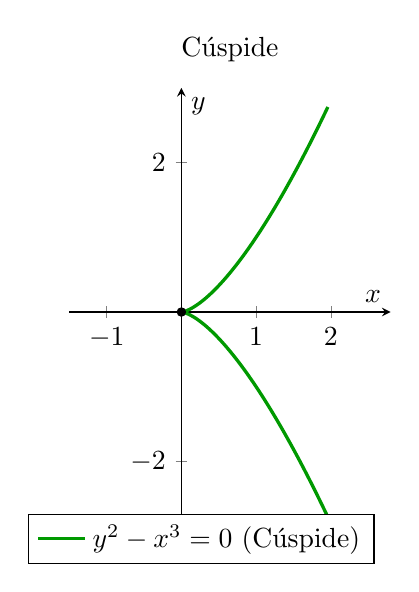
\begin{tikzpicture}
    \begin{axis}[
        axis lines = center,
        xlabel = $x$, ylabel = $y$,
        xmin = -1.5, xmax = 2.8, % Límites ajustados ligeramente
        ymin = -3.0, ymax = 3.0, % Límites Y aumentados para la cúspide
        axis equal image,
        %grid = major,
        legend style={at={(0.95,0.05)},anchor=north east}, % Leyenda arriba a la derecha
        title = {Cúspide}
    ]

    % --- CURVA 3: Cúbica Cuspidal (Cúspide) ---
    % Ecuación: y^2 - x^3 = 0
    % Parametrización: x = t^2, y = t^3
    % Usamos un dominio para 't' tal que t^2 no exceda demasiado el xmax
    \addplot [
        domain=-1.4:1.4,  % t=1.4 -> x=1.96, y=2.74
        samples=200, 
        color=green!60!black, % Verde oscuro
        very thick
    ] ({x^2}, {x^3});
    \addlegendentry{$y^2 - x^3 = 0$ (Cúspide)}

    % Decoración: Marcar el origen donde coinciden la cúspide y el nodo
    \addplot[mark=*, color=black, mark size=1.5pt] coordinates {(0,0)};

    \end{axis}
\end{tikzpicture}$$
    Sea $k$ cuerpo algebraicamente cerrado ($k = \bb C$), el polinomio $y^2-x^3$ es irreducible, 
    $$Spec \,\,  \modulo{k[x,y]}{(y^2-x^3)} = \begin{cases}
        0  \\ \m_{\alpha, \beta}=(x-\alpha, y-\beta) & / P(\alpha, \beta)=0, \,  \alpha, \beta\in k  
    \end{cases}$$
    con el morfismo 
    $$\bt \modulo{k[x,y]}{(y^2-x^3)} \rar{\phi} & k \\[-5mm] x \rarmaps & \alpha \\[-5mm] y \rarmaps & \beta \et$$
    de forma que $\ker \phi = \m_{(\alpha, \beta)}$, lo que nos da la sucesi\'on exacta
    $$\bt 0\rar & \m_{(\alpha, \beta)} \rar & \modulo{k[x,y]}{(y^2-x^3)} \rar & k \rar 
    & 0 \et$$



    %25/11/2025

    Vamos a localizar sobre los ideales primos de $Spec$.
    
    De esta forma, $A_0 = \Sigma$ es el cuerpo de fracciones de $A$, y as\'i
    $$\Omega_{\nicefrac{A}{k}} \underset{A}{\otimes} \Sigma = \modulo{\Sigma \, dx \oplus \Sigma \, dy}{\langle -3x^2 \, dx +2y \, dy \rangle}$$
    y si $ch(k)\neq 3$ (si $ch(k) = 3, \, ch(k)\neq 2$ pudiedo despejar $dy$ en vez de $dx$), $dx= \frac{2y}{3x} \, dy$, luego
    $$\Omega_{\nicefrac{A}{k}} \underset{A}{\otimes} \Sigma = \modulo{\Sigma \, dx \oplus \Sigma \, dy}{\langle -3x^2 \, dx +2y \, dy \rangle} = \Sigma \, dy$$
    que es un $\Sigma$-espacio vectorial de dimensi\'on 1. 
\end{ejem}
\begin{prop} Sea $A$ una $k$-\'algebra, $S\subseteq A$ un sistema multiplicativo, $k \to A \to A_S$,
      $$\Omega_{\nicefrac{A}{k}} \underset{A}{\otimes} S = \Omega_{\nicefrac{A_S}{k}}$$
      es decir, que las diferenciales conmutan con la localizaci\'on.
\end{prop}
\begin{dem}
    Tenemos el morfismo 
    $$\bt \Omega_{\nicefrac{A}{k}} \underset{A}{\otimes} S \rar & \Omega_{\nicefrac{A_S}{k}} \et$$
    y para ver que es un isomorfismo basta ver que al tomar $Hom_{A_S}(-,M)$ es isomorfismo ($\forall \, M$ $A_S$-m\'odulo).
    $$\bt Hom_{A_S}(\Omega_{\nicefrac{A_S}{k}} , M)\rar &Hom_{A_S}( \Omega_{\nicefrac{A}{k}} \underset{A}{\otimes} S, M) \\[-5mm] & \arrow[equal]{u} Hom_{A}(\Omega_{\nicefrac{A}{k}} , M) \\[-5mm] Der_k(A_S,M) \arrow[equal]{uu} \rar & \arrow[equal]{u} Der_k(A,M) \\[-5mm] \tilde D \rarmaps & \tilde D \circ i \et$$
    que es el morfismo dado por el diagrama
    $$\bt A \rar{i} \arrow{dr} & A_S \arrow[dashed]{d}{\tilde D} \\[3mm] & M \et$$

    Para ver que es isomorfismo, veamos que dada $D:A\longrightarrow M$ existe una \'unica $\tilde D: A_S \longrightarrow M$ asociada, haciendo el tri\'angulo anterior conmutativo. 

    Supongamos que ya tenemos $\tilde D$, veamos cu\'anto vale aplicado a $\frac{a}{s}$:
    $$\tilde D\left( \frac{a}{s} \right) = \tilde  D\left(  \frac{1}{s}\cdot \frac{a}{1} \right)= \frac{1}{s}\cdot \tilde   D\left(  \frac{a}{1} \right) + \frac{a}{1} \cdot  \tilde  D\left(  \frac{1}{s} \right) = \frac{1}{s} D(a) - \frac{a}{1} \cdot \frac{1}{s^2} \, D(s) = \frac{s \, Da - a \, Ds}{s^2}$$
    por ser
    $$0 = \tilde D(1) = \tilde  D\left(  \frac{s}{s} \right) = \tilde  D\left(  \frac{1}{s}\cdot \frac{s}{1} \right) = \frac{1}{s} \, D(s) + \frac{s}{1} \tilde  D\left(  \frac{1}{s} \right) \Rightarrow  \tilde  D\left(  \frac{1}{s} \right) = - \frac{1}{s^2} \, D(s) $$

    Y tenemos $\tilde D$ determinada por la $D$, siendo \'unica. Debemos probar que esta definici\'on no depende del representante elegido de $\frac{a}{s}$, es decir, que si hacemos con $\frac{a'}{s'} \sim \frac{a}{s}$ obtenemos el mismo resultado. Adem\'as, se comprueba que es $k$-lineal y que es una derivaci\'on, es decir que cumple la regla de Leibnitz. Adem\'as, $\tilde D(\nicefrac{a}{1}) = Da$ por la definici\'on.
\end{dem}
\begin{cor}
          $\Omega_{\nicefrac{A}{k}} \underset{A}{\otimes} \Sigma = \Omega_{\nicefrac{\Sigma}{k}}$
\end{cor}
\begin{obs}
    Tenemos la regla de c\'alculo 
    $$\tilde D\left( \frac{a}{s} \right)  = \frac{s \, Da - a \, Ds}{s^2}$$
\end{obs}
\begin{ejem}
    Continuando con el ejemplo anterior, $\m_{(\alpha, \beta)} = (x-\alpha, y-\beta)$, ten\'iamos el morfismo, por el punto racional, 
    $$\bt k \arrow[bend left=10mm, equal]{rr} \rar[hook] & A \rar & \modulo{A}{\m_{(\alpha, \beta)}} = k\\[-5mm] & x \rarmaps & \alpha \\[-5mm] & y \rarmaps & \beta \et$$
    luego 
    $$\Omega_{\nicefrac{A}{k}} \underset{A}{\otimes} \modulo{A}{\m_{(\alpha, \beta)}} = \modulo{k \, dx \oplus k \, dy}{\langle -3\alpha^2 \, dx +2\beta\,  dy \rangle} =$$
    $$=\begin{cases}
        \text{ de } \dim 2: -3\alpha^2 = 0 \text{ y } 2 \beta =0 \Rightarrow \alpha=0, \, \beta =0 & \m_{(0,0)} = (x,y) \\  \text{ de } \dim 1:\,  (\alpha, \beta) \neq (0,0)
    \end{cases} $$
    y por otro lado, 
    $$\Omega_{\nicefrac{A}{k}} \underset{A}{\otimes} \modulo{A}{\m_{(\alpha, \beta)}} = \modulo{\m_{(\alpha, \beta)}}{\m^2_{(\alpha, \beta)}}$$ y esto nos dice que, al localizar por $\m_{(\alpha, \beta)}$, $A \longrightarrow A_{\m_{(\alpha, \beta)}}$, su espectro va a ser un \'unico maximal, eliminando el resto de maximales, de forma que hemos localizado el anillo, siendo el \'unico maximal $\m_{(\alpha, \beta)} A_{\m_{(\alpha, \beta)}}$. 

    Ten\'iamos que $\m_{(0,0)} = (x,y)$ en $A_{\m_{(0,0)}}$ y no es prinicipal, pues $\modulo{\m_{(\alpha, \beta)}}{\m^2_{(\alpha, \beta)}}$ es de $\dim 2$. En otro caso, si $(\alpha, \beta)\neq(0,0)$, $\m_{(\alpha, \beta)} = (x-\alpha, y-\beta)$ en $A_{\m_{(\alpha, \beta)}}$ es principal, es decir, est\'a generado por un elemento, por ser $\modulo{\m_{(\alpha, \beta)}}{\m^2_{(\alpha, \beta)}}$ es $\dim 1$. 
\end{ejem}
\begin{ejem}
    Consideremos en $\bb R^2$ el eje de abcisas, con el morfismo de proyectivizaci\'on
    $$\bt \bb R^2\rar & \bb R \\[-5mm] (\alpha,\beta) \rarmaps & \alpha \et$$
    donde el plano va a ser $k[x,y]$, y cada punto es un morfismo epiyectivo de $k$-\'algebras, es decir, un ideal primo maximal y racional
    $$\bt 0\rar & \m_{(\alpha, \beta)} \rar & k[x,y] \rar & k \rar & 0 \\[-5mm] 
    & (x-\alpha, y-\beta) \arrow[equal]{u} &  &
    \et$$
    y la recta del eje de abcisas es $k[x]$, con 
    $$\bt 0\rar & (x-\alpha) \rar & k[x] \rar & k \rar & 0\\[-5mm] & &x\rarmaps & \alpha   \et$$
    y el morfismo de proyectivizaci\'on va a ser un morfismo de $k$-\'algebras
    $$\bt k[x] \rar & k[x,y] \\[-5mm] x\rarmaps & x \et$$
    Calculemos $\Omega_{\nicefrac{k[x,y]}{k[x]}}$. Por la 1ª sucesi\'on exacta, 
    $$\bt \Omega_{\nicefrac{k[x]}{k}} \underset{k[x]}{\otimes} k[x,y] \rar & \Omega_{\nicefrac{k[x,y]}{k}} \rar & \Omega_{\nicefrac{k[x,y]}{k[x]}} \rar & 0 \\[-5mm] k[x,y] \, dx \arrow[equal]{u} \rar & \arrow[equal]{u} k[x,y] dx \oplus k[x,y] dy & k[x,y] \, dy \arrow[equal]{u}  \\[-5mm] dx \rarmaps & dx \et$$
    Otra forma hubiera sido hacer $k[x,y]= k[x][y] = A[y]$, de forma que $\Omega_{\nicefrac{A}{k}} = $
\end{ejem}
\begin{ejem}
    Consideremos $C = \{x^2+y^2-1=0\} = \{(\alpha, \beta) \in k\times k\, : \, \alpha^2+\beta^2-1=0\}$, de forma que
    $$\bt \modulo{k[x,y]}{(x^2+y^2-1)} \rar & k \\[-5mm] x \rarmaps & \alpha \\[-5mm] x \rarmaps & \beta \\[-5mm] 0 =x^2+y^2-1 \rarmaps & \alpha^2+\beta^2-1=0 \et$$
    est\'a bien definido. De esta forma, los puntos racionales del anillo $ \modulo{k[x,y]}{(x^2+y^2-1)}$ son los de la circunferencia. 

    Tenemos 
    $$\bt k[x] \arrow[bend left=10mm]{rr} \rar[hook] & k[x,y] \rar &  \modulo{k[x,y]}{(x^2+y^2-1)} \et$$
    de forma que la proyecci\'on $C \longrightarrow k$ es el morfismo anterior $k[x] \longrightarrow  \modulo{k[x,y]}{(x^2+y^2-1)}$. Vamos a calcular $\Omega_{\modulo{\nicefrac{k[x,y]}{(x^2+y^2-1)}}{k[x]}}$. Sea $k[x] \longrightarrow A=  \modulo{k[x,y]}{(x^2+y^2-1)}$, por la 1ª sucesi\'on exacta, 
    $$\bt \Omega_{\nicefrac{k[x]}{k}} \underset{k[x]}{\otimes} A \rar & \Omega_{\nicefrac{A}{k}} \rar & \Omega_{\nicefrac{A}{k[x]}} \rar & 0 \\[-5mm] 
    \arrow[equal]{u} k[x]dx \underset{k[x]}{\otimes} A = Adx \rar  & \arrow[equal]{u} \modulo{Adx\oplus Ady}{\cancel{2}x \, dx + \cancel{2}y\, dy} & \arrow[equal]{u} \modulo{Ady}{\langle y \, dy \rangle} = \modulo{A}{(y)} \, dy \\[-5mm] & & \arrow[equal]{u}  \modulo{k[x,y]}{(x^2+y^2-1, \, y)} \\[-5mm] & & \arrow[equal]{u} \modulo{k[x]}{x^2-1} \et$$
    si $ch(k)\neq 2$. Entonces, las diferenciales relativas nos da $\modulo{k[x]}{x^2-1}$, cuyos puntos racionales nos dicen los puntos de $C$ en los que la direcci\'on de proyecci\'on es tangente. 

    De otro modo, sea $\bar k = k[x] \longrightarrow  \modulo{k[x,y]}{(x^2+y^2-1)} = \modulo{\bar k[y]}{(x^2+y^2-1)}$, y entonces ten\'iamos que
    $$\Omega_{\modulo{(\nicefrac{k[x]}{(P)})}{k}} = \modulo{k[x]}{(P,P')} dx$$
    luego 
    $$\Omega_{\modulo{( \nicefrac{k[x,y]}{(x^2+y^2-1)})}{\bar k}} = \modulo{\bar k[y]}{(x^2+y^2-1,\, \cancel{2}y)} dy$$
\end{ejem}
\begin{ejem}
    Sea $P(x,y)=0$, es una curva en $k\times k$, y $Q(x,y)=0$ otra curva. Los puntos donde se cortan ambas son los puntos racionales de $A=\modulo{k[x,y]}{(P,Q)}$, es decir, las soluciones de $\{P=0, \, Q=0\}$. Supongamos que $P$ y $Q$ no tienen factores comunes. Entonces las soluciones de $P=Q$ son un n\'umero finito. 

    Calculemos las diferenciales de $A$: $ \Omega_{\nicefrac{A}{k}}=\Omega_{\modulo{(\nicefrac{k[x,y]}{(P,Q)})}{k}} $. En general, usando la 2ª sucesión exacta, llamando $I=(P,Q)$, 
    $$\bt \modulo{I}{I^2} \rar &  \Omega_{\nicefrac{k[x,y]}{k}} \underset{k[x,y]}{\otimes} A \rar & \Omega_{\nicefrac{A}{k}} \rar & 0 \\[-5mm] \modulo{(P,Q)}{(P,Q)^2} \rar \arrow[equal]{u} & Adx\oplus Ady \arrow[equal]{u} &  \\[-5mm] P \rarmaps & dP \\[-5mm] Q \rarmaps & dQ  \et$$
    en definitva, 
    $$\Omega_{\nicefrac{A}{k}} = \modulo{Adx\oplus Ady}{\langle dP, \, dQ \rangle}$$
\end{ejem}
\begin{ejem}
    Consideremos $A=\modulo{k[x,y]}{(x^2+y^2-1, y^2-x^2-x^3)}$
    $$\Omega_{\nicefrac{A}{k}} = \modulo{Adx\oplus Ady}{\langle xdx+ydy, -(2x+3x^2)dx + 2ydy \rangle}$$
$$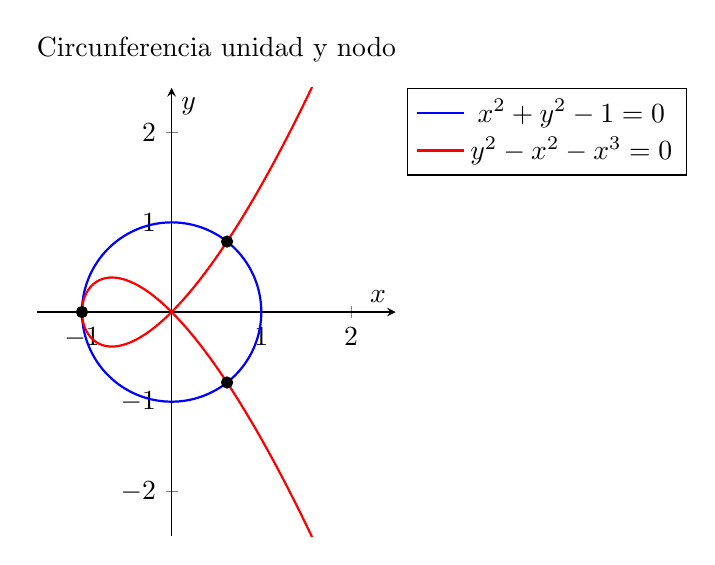
\begin{tikzpicture}
    \begin{axis}[
        axis lines = center,     % Ejes centrados en el origen
        xlabel = $x$,
        ylabel = $y$,
        xmin = -1.5, xmax = 2.5, % Límites del eje X
        ymin = -2.5, ymax = 2.5, % Límites del eje Y
        axis equal image,        % Mantiene la proporción 1:1 (para que el círculo sea redondo)
        %grid = major,            % Cuadrícula de fondo
        legend pos = outer north east, % Leyenda fuera del gráfico
        title = {Circunferencia unidad y nodo}
    ]

    % 1. El Círculo Unitario: x^2 + y^2 - 1 = 0
    % Parametrización: x = cos(t), y = sin(t)
    \addplot [
        domain=0:360, 
        samples=200, 
        color=blue, 
        thick
    ] ({cos(x)}, {sin(x)});
    \addlegendentry{$x^2 + y^2 - 1 = 0$}

    % 2. La Curva Cúbica (Tschirnhausen): y^2 - x^2 - x^3 = 0
    % Parametrización: x = t^2 - 1, y = t^3 - t
    % Usamos 'x' en el dominio para representar el parámetro 't'
    \addplot [
        domain=-1.8:1.8, 
        samples=200, 
        color=red, 
        thick
    ] ({x^2 - 1}, {x^3 - x});
    \addlegendentry{$y^2 - x^2 - x^3 = 0$}

    % Puntos de intersección (Opcional, para decoración)
    % Se cruzan en x=-1 y x approx 0.618
    \addplot[mark=*, color=black, only marks] coordinates {(-1,0) (0.618, 0.786) (0.618, -0.786)};

    \end{axis}
\end{tikzpicture}$$
y se tiene la sucesi\'on exacta, para un punto racional $(x-\alpha, y-\beta)$
$$\bt 0 \rar & \m_{(\alpha, \beta)} \rar & A \rar & k = \modulo{A}{\m_{(\alpha, \beta)} } \rar & 0 \\[-5mm] 
        & (x-\alpha, y-\beta) \arrow[equal]{u} & x\rarmaps & \alpha \\[-5mm] & & y\rarmaps & \beta 
\et$$
verificando las relaciones $\alpha^2+ \beta^2-1=0, \, \beta^2 - \alpha^2 - \alpha^3 =0$, de forma que
$$\Omega_{\nicefrac{A}{k}} \underset{A}{\otimes} \modulo{A}{ \m_{(\alpha, \beta)} } = \modulo{kdx\oplus kdy}{ \langle  2\alpha dx + 2\beta dy, \, -(2\alpha+3\alpha^2) dx+2\beta dy\rangle}$$
de forma que este es un $k$-espacio vectorial, y para que sea nulo, tienen que ser linealmente independientes, es decir, para que sea no nulo, deben ser dependientes.

Supongamos $ch(k)\neq 2$, los vectores por los que hacemos cociente tiene coordenadas $(\alpha, \beta), \, (-(2\alpha+3\alpha^2), \, 2\beta)$, y para que sean linealmente independientes, usamos el determinante
$$\left|\begin{matrix}
    \alpha & \beta \\ -(2\alpha+3\alpha^2) & 2\beta 
\end{matrix} \right| = 2\alpha \beta + \beta \alpha (2+3\alpha) = \alpha\beta (4+3\alpha) = 0 \iff \begin{cases}
    \alpha=0 \\ \beta =0 \\ 4+3\alpha=0
\end{cases}$$
Sutituyendo en las ecuaciones de las curvas, si $\alpha=0$, $\beta=0,\beta=\pm 1$, sin soluci\'on, y de la misma forma $4+3\alpha$ hace que $\beta$ no tiene soluci\'on. Si $\beta = 0$, $\alpha=-1$, y aqu\'i las diferenciales no son 0. 
\end{ejem}
\begin{ejem}
    En general, para cualquier curva $f(x,y)=0$, la recta tangente en $(\alpha, \beta)$ es 
    $$\pd{f}{x}\Big|_{(\alpha,\beta)}(x-\alpha) + \pd{f}{y}\Big|_{(\alpha,\beta)}(y-\beta)$$

    Si tenemos $f: \bb R \longrightarrow \bb R$, $x \longmapsto f(x)$ tenemos la gr\'afica de $x$, con su $F(x,y) = y-f(x)$. Para cualquier punto de la gr\'afica $(\alpha, f(\alpha))$, la recta tangente es
    $$0=\pd{F}{x}\Big|_{(\alpha, f(\alpha))} (x-\alpha) + \pd{F}{y}\Big|_{(\alpha, f(\alpha))} (y-f(\alpha)) = -f'(\alpha)(x-\alpha) + (y-f(\alpha)) $$
    $$\Rightarrow y-f(\alpha) = f'(\alpha) (x-\alpha) $$
\end{ejem}
\begin{ejem}
    Si trabajamos sobre la $k$-\'algebra $A = \modulo{k[x,y]}{(P(x,y))}$, 
    $$\Omega_{\nicefrac{A}{k}} = \modulo{Adx\oplus Ady}{\langle \pdd{P}{x}dx+ \pdd{P}{y} dy \rangle}$$
    y si las calculamos en un punto de la curva
    $$\Omega_{\nicefrac{A}{k}} \underset{A}{\otimes} \modulo{A}{\m_{(\alpha,\beta)}} = \modulo{kdx \oplus k dy}{\left\langle \pdd{f}{x}|_{(\alpha,\beta)} dx + \pdd{f}{y}|_{(\alpha,\beta)}dy \right\rangle} $$
    y para que sea de dimensi\'on 1, el vector por el que hacemos cociente debe ser distinto de 0, es decir, no se anulan a la vez
\end{ejem}
\begin{defi}
    Decimos que $(\alpha, \beta)$ es no singular si $\pd{f}{x}\Big|_{(\alpha,\beta)} dx + \pd{f}{y}\Big|_{(\alpha,\beta)}dy \neq 0$, es decir, si $\pd{f}{x}\Big|_{(\alpha,\beta)} \neq 0$ \'o $\pd{f}{y}\Big|_{(\alpha,\beta)} \neq 0$.
\end{defi}
\begin{ejem}
    Si tenemos ahora $A = \modulo{k[x,y]}{(P,Q)}$ 
    $$\Omega_{\nicefrac{A}{k}}= \modulo{Adx\oplus Ady}{\langle \pdd{P}{x} dx+\pdd{P}{y}dy, \pdd{Q}{x} dx+\pdd{Q}{y}dy \rangle}$$
    y consideramos $(\alpha, \beta)$ tal que $P(\alpha, \beta) = 0 = Q(\alpha, \beta)$, y hacemos
    $$\Omega_{\nicefrac{A}{k}} \underset{A}{\otimes} \modulo{A}{ \m_{(\alpha, \beta)} } = \modulo{kdx\oplus kdy}{ \left\langle  \pdd{P}{x}|_{(\alpha,\beta)} dx+\pdd{P}{y}|_{(\alpha,\beta)}dy, \, \pdd{Q}{x}|_{(\alpha,\beta)} dx+\pdd{Q}{y}|_{(\alpha,\beta)}dy   \right\rangle}$$
    de forma que para estudiar cuando se anula usamos el jacobiano
    $$ \left| \begin{matrix}
         \pdd{P}{x} & \pdd{P}{y} \\ \pdd{Q}{x} & \pdd{Q}{y} 
    \end{matrix} \right|_{(\alpha, \beta)}$$
    y si $(\alpha, \beta)$ es singular, $\Omega_{\nicefrac{A}{k}} \underset{A}{\otimes} \modulo{A}{ \m_{(\alpha, \beta)} } \neq 0$. En otro caso, si el punto no es singular, ninguno de los vectores del cociente son 0, que las diferenciales en ese punto sea distintas de 0 implica que las tangentes son la misma.
\end{ejem}
\begin{ejem}
    Si $A = \modulo{k[x,y,z]}{(P)}$, ser\'a una superficie
    $$\Omega_{\nicefrac{A}{k}} = \modulo{Adx\oplus Ady \oplus Adz}{\langle dP\rangle}$$ con $(\alpha,\beta, \gamma)\, : \, P(\alpha,\beta, \gamma)=0$ se tiene el morfismo racional que induce la s.e.
    $$\bt 0 \rar & \m_{(\alpha,\beta, \gamma)} \rar & A \rar & k \rar & 0\\[-5mm] & \arrow[equal]{u} (x-\alpha,y-\beta,z-\gamma) \et$$
    y las diferenciales en el punto
    $$\Omega_{\nicefrac{A}{k}} \underset{A}{\otimes} \modulo{A}{ \m_{(\alpha, \beta)} } = \modulo{kdx\oplus kdy}{ \langle  \pdd{P}{x}|_{(\alpha, \beta, \gamma)} dx+\pdd{P}{y}|_{(\alpha, \beta, \gamma)}dy +\pdd{P}{z}|_{(\alpha, \beta, \gamma)}dz    \rangle}$$
    es de dim 2 o 3, ser\'a 3 cuando las parciales se anulen. En otro caso, lo que tenemos es el espacio tangente, y para $(\alpha,\beta, \gamma)$, se tiene el plano tangente  
    $$\pdd{P}{x}\Big|_{(\alpha, \beta, \gamma)} (x-\alpha)+\pdd{P}{y}\Big|_{(\alpha, \beta, \gamma)} (y-\beta) +\pdd{P}{z}\Big|_{(\alpha, \beta, \gamma)} (z-\gamma)$$
\end{ejem}

